\documentclass[pdftex]{beamer}
%\documentclass[notes=show]{beamer}
%\documentclass[xcolor=dvipsnames]{beamer}

\usepackage{amssymb}
\usepackage{latexsym}
\usepackage{amsfonts}
\usepackage{amsmath}
\usepackage[absolute,overlay]{textpos}
\usepackage[english]{babel}
\usepackage[latin1]{inputenc}
%\usepackage{times}
\usepackage[T1]{fontenc}
\usepackage{tabularx}
\newcolumntype{Y}{>{\small\raggedright\arraybackslash}X}
\usepackage{graphicx}
\usepackage{bigstrut}
\usepackage{bbm}
\usepackage{mathrsfs}
\usepackage{epsfig}
\usepackage{array}
%\usepackage{natbib}

\mode<presentation> {
%\usetheme[left,width=1.7cm]{Berkeley}
%\usetheme{default}
\usetheme{Boadilla}
  \usecolortheme[RGB={103,102,204}]{structure}
%\usecolortheme{dove}
  \useoutertheme{infolines}
  \setbeamercovered{transparent}
 }

%\renewcommand{\familydefault}{cmss}
%\renewcommand{\mathrm}{\mathsf}
%\renewcommand{\textrm}{\textsf}
\usefonttheme{serif}
\newcommand{\X}{{\mathbf{X}}}
\newcommand{\x}{{\mathbf{x}}}
\newcommand{\E}{\mathsf{E}}
\newcommand{\V}{\mathsf{Var}}


    %%%%%%%%%%%%%%%%%%%%%%%%%%%%%%%%%%%%%%%%%%%%%%%%%%%%%%%%%%%%%%%%%%%%%%%%%%%%%%
    %         Neue Kommandos f�r fette Mathebuchstaben innerhalb von Formeln     %
    %%%%%%%%%%%%%%%%%%%%%%%%%%%%%%%%%%%%%%%%%%%%%%%%%%%%%%%%%%%%%%%%%%%%%%%%%%%%%%
    \newcommand{\bom}{\boldmath}
    \newcommand{\ubom}{\unboldmath}
    \newcommand{\mb}{\mathbf}

    \newcommand{\fmalpha}{\mbox{\bom${\alpha}$}}               %Fettes alpha
    \newcommand{\fmbeta}{\mbox{\bom${\beta}$}}                 %Fettes beta
    \newcommand{\fmgamma}{\mbox{\bom${\gamma}$}}               %Fettes gamma
    \newcommand{\fmdelta}{\mbox{\bom${\delta}$}}               %Fettes delta
    \newcommand{\fmepsilon}{\mbox{\bom${\epsilon}$}}           %Fettes epsilon
    \newcommand{\fmvarepsilon}{\mbox{\bom${\varepsilon}$}}     %Fettes varepsilon
    \newcommand{\fmzeta}{\mbox{\bom${\zeta}$}}                 %Fettes zeta
    \newcommand{\fmeta}{\mbox{\bom${\eta}$}}                   %Fettes eta
    \newcommand{\fmta}{\mbox{\bom${\theta}$}}                  %Fettes theta (ta)
    \newcommand{\fmvarta}{\mbox{\bom${\vartheta}$}}         	 %Fettes vartheta (ta)
    \newcommand{\fmiota}{\mbox{\bom${\iota}$}}                 %Fettes iota
    \newcommand{\fmkappa}{\mbox{\bom${\kappa}$}}               %Fettes kappa
    \newcommand{\fmla}{\mbox{\bom${\la}$}}                     %Fettes lambda (la)
    \newcommand{\fmmu}{\mbox{\bom${\mu}$}}                     %Fettes mu
    \newcommand{\fmnu}{\mbox{\bom${\nu}$}}                     %Fettes nu
    \newcommand{\fmxi}{\mbox{\bom${\xi}$}}                     %Fettes xi
    \newcommand{\fmo}{\mbox{\bom${\o}$}}                       %Fettes o
    \newcommand{\fmpi}{\mbox{\bom${\pi}$}}                     %Fettes pi
    \newcommand{\fmvarpi}{\mbox{\bom${\varpi}$}}               %Fettes varpi
    \newcommand{\fmrho}{\mbox{\bom${\rho}$}}                   %Fettes rho
    \newcommand{\fmvarrho}{\mbox{\bom${\varrho}$}}             %Fettes varrho
    \newcommand{\fmsigma}{\mbox{\bom${\sigma}$}}               %Fettes sigma
    \newcommand{\fmvarsigma}{\mbox{\bom${\varsigma}$}}         %Fettes varsigma
    \newcommand{\fmtau}{\mbox{\bom${\tau}$}}                   %Fettes tau
    \newcommand{\fmupsilon}{\mbox{\bom${\upsilon}$}}           %Fettes upsilon
    \newcommand{\fmphi}{\mbox{\bom${\phi}$}}                   %Fettes phi
    \newcommand{\fmvarphi}{\mbox{\bom${\varphi}$}}             %Fettes varphi
    \newcommand{\fmchi}{\mbox{\bom${\chi}$}}                   %Fettes chi
    \newcommand{\fmpsi}{\mbox{\bom${\psi}$}}                   %Fettes psi
    \newcommand{\fmomega}{\mbox{\bom${\omega}$}}               %Fettes omega
    \newcommand{\fmimath}{\mbox{\bom${\imath}$}}               %Fettes imath


\setbeamercolor{bibliography entry title}{fg=black}
\setbeamercolor{bibliography entry author}{fg=black}
\setbeamercolor{subsection in toc}{fg=structure}
\setbeamercolor{palette primary}{bg=structure, fg=white}
%\setbeamercolor{palette secondary}{bg=structure, fg=black}
%\setbeamercolor{palette tertiary}{bg=structure, fg=black}
\setbeamercolor{caption name}{fg=black} \setbeamersize{text margin
left=.8cm} \setbeamersize{text margin right=1cm}
\hypersetup{linkbordercolor={1 0 0}} \setbeamertemplate{navigation
symbols}{} \setbeamertemplate{headline}[default]

\setbeamertemplate{enumerate items}[default]

\newcounter{transfct}
\newcounter{begbs}
\newcounter{endbs}
\title[Introduction]{Econometrics 2 (Part 1)}

\author[Weber  \& Mu\c co]{Arieda Mu\c co}
\institute[CEU]{Central European University}
\date{Winter 2018}


\AtBeginSection[] {
  \begin{frame}<handout:0>
    \frametitle{TOC}
    \tableofcontents[currentsection]
  \end{frame}
}

%\AtBeginSubsection[] {
%  \begin{frame}<beamer>
%   \frametitle{Outline}
%    \tableofcontents[currentsection,currentsubsection]
%  \end{frame}
%}

%\beamerdefaultoverlayspecification{<+->}

\pgfdeclareimage[height=.7cm]{logo}{rgs2}
\logo{\pgfuseimage{logo}}
\begin{document}

\frame{\titlepage}


\begin{frame}
\frametitle{Contact}
\begin{itemize}
\item Andrea Webber: \href{mailto:WebberA@ceu.edu}{WebberA@ceu.edu}\\
Office: Nador 13, 513
\item Arieda Mu\c co: \href{mailto:MucoA@ceu.edu}{MucoA@ceu.edu}\\
Office: Nador 13, 507
\item Istvan Boza (TA): \href{mailto:boza_istvan@phd.ceu.edu}{boza\_istvan@phd.ceu.edu}
\end{itemize}

\end{frame}

\begin{frame}
\frametitle{Textbooks}
\begin{itemize}
\item Wooldridge, Introductory Econometrics: A Modern Approach
\item Angrist and Pischke, Mostly Harmless Econometrics
\item Reading list of applied papers
\end{itemize}
\end{frame}




\begin{frame}
\frametitle{Applied Microeconometrics}

\begin{itemize}
\item Investigate micro-econometric methods and research designs

\item Discuss applied research papers - learn from good examples

\item Perform own empirical exercises based on data (real and simulated)

\item Topics: Labor, Population, Health, Public,  Development, and Political Economics

\end{itemize}
\end{frame}




\begin{frame}
\frametitle{TA Sessions}
\begin{itemize}
\item Six TA session
\item You are encouraged to work in groups, but every student hands in individual solutions
\item Solutions have to be turned in at specified dates (via Moodle)
\item Problem sets mostly replicate and discuss estimation results
\begin{itemize}
\item Provided with datasets
\end{itemize}
\end{itemize}
\end{frame}



\begin{frame}
\frametitle{Stata License}
\begin{itemize}
\item CEU lab
\item Problem-sets are going to be using STATA
\item Knowledge of STATA is not a prerequisite 
\item Short STATA intro in the first TA session
\end{itemize}
\end{frame}



\begin{frame}
\frametitle{Course Goals}
Guidance for conducting sensible applied research projects

\begin{enumerate}
\item Formulate research question

\item Find data

\item Econometric method, statistical analysis

\item Interpret estimation results

\item Policy recommendations
\end{enumerate}
\end{frame}



\begin{frame}
\frametitle{Grading}
\begin{itemize}
\item \textbf{Problem Sets} (20\% of final grade)
\item  \textbf{Term paper} (30\% of final grade)
\item \textbf{Final Exam}  (50\% of final grade)
\begin{itemize}
\item The exam will be closed book, closed notes
\item Cover the material presented in class and seminars
\item Questions which require short answers
\end{itemize}
\end{itemize}
\end{frame}



\begin{frame}
\frametitle{Term Paper}
\begin{itemize}
\item An individual term paper is required at the end of the course
\item The paper should consist of a simple empirical analysis
\begin{itemize}
\item It should be at most 10 pages long (including tables and figures), text 1.5 or double spaced, font size 12
\end{itemize}
\item There will be three deadlines
\begin{itemize}
\item Submit a research proposal via Moodle
\item Hand in the first draft for review at the Center for Academic Writing
\item Upload in Moodle the final version in \textbf{.pdf} format. The file should be named as: \emph{name\_surname\_project.pdf}
\end{itemize}

\end{itemize}
\end{frame}



\begin{frame}
\frametitle{Outline: Tentative Schedule and Reading List}
\begin{enumerate}
\item Economic research questions: causality
\item The experimental ideal
\item Linear regression
\item Instrumental Variables
\item Panel Data, Fixed Effects, Differences-in-Differences
\item Program Evaluation: Nonparametric Methods
\item Regression Discontinuity
\end{enumerate}
\end{frame}

\begin{frame}
\frametitle{Research Questions }
\begin{enumerate}
\item What is the relationship of interest
\begin{itemize}
\item Descriptive research
\item Causal inference
\begin{itemize}
\item A causal relationship is useful for making predictions about the consequences of changing circumstances
\item i.e Effect of education on wages, effect of class size on student achievement, deworming on education and health, institutions on growth ...
\end{itemize}
\end{itemize}

\item Which experiment could be ideally used?
\begin{itemize}
\item Often hypothetical but helps formulating the question
\end{itemize}
\item What is the identification strategy?
\item What is the mode of statistical inference?
\end{enumerate}
\end{frame}

\begin{frame}
\frametitle{ Experimental data}
Hard and costly to obtain.
    \begin{itemize}
    \item Controlled laboratory experiment 
    \item Randomized controlled trials
    \end{itemize}
Give one extra year of education to a randomly selected group and compare means in the treatment and control group.
 Due to randomization the extra year is unrelated to parents education, neighbourhood income, etc
 \end{frame}

 
 \begin{frame}
\frametitle{Non-experimental data - Observational data}
	
    \begin{itemize}
    \item Cross sectional data - sample of units taken at a given point in time, random sampling
    \item Time series data - one variable observed over time, observations in general not independent over time
    \item Pooled cross sections
    \item Panel data - a time series for each cross-sectional unit
    \end{itemize}
People choose to go to university. Choice depends on other factors affecting wage. Difficult to unbundle effects.
Try to find variation of years of schooling which is random. Try to account for other factors: controls.
\end{frame}

%\frame{ \frametitle{}
%\begin{center}
%\begin{figure}
%
\includegraphics[width=0.8\linewidth]{graphs/detective.png}
%\end{figure}
%\end{center}
 %}
 
\begin{frame}
\frametitle{Statistical Models of Shoe and Leather}
Freedman, David A. (1991) "Statistical Models and Shoe Leather", Sociological Methodology, 21, 291-313
\bigskip

John Snow studies of the cholera epidemics in Europe in the 19th century and proves that cholera is a waterborne infectious disease

\begin{itemize}
  \item In the $19^{th}$ century no microbiology, limited microscopes
  \item Theory: diseases result from "poison in the air" - miasma
  \item Cholera Europe in epidemic waves
  \item Snow studied spatial pattern of epidemics along tracks of human commerce
  \item Influence of water supply on incidence of Cholera?
\end{itemize}
\end{frame}

\begin{frame}
\frametitle{Scientific Detective Work}
Is cholera a waterborne or an airborne disease?
\bigskip

London in the 1800's: different water companies serve different areas

\begin{itemize}
  \item Some companies take water from the Thames polluted by sewage
  \item 2 companies
  \begin{itemize}
  \item Southwark \& Vauxhall: downstream from sewage discharges
  \item Lambeth: intake point upstream
  \end{itemize}

  \item Both companies served the same parts of London during the 1853-54 cholera epidemic
  \item Sometimes houses next to each other in the same street were served by the 2 different companies
    \begin{itemize}

  \item Each company supplies rich and poor, large and small houses, no difference in condition or occupation
  \end{itemize}
  \item Idea: compare number of cholera victims
\end{itemize}
\end{frame}

\begin{frame}
\frametitle{Method of Shoe and Leather}

\begin{itemize}
  \item Snow surveyed houses in large parts of London
  \item Water company
  \item Cholera victims
  \item 300,000 households involved
  \item Reward: clear result
\end{itemize}
\end{frame}

 \frame{ \frametitle{}
\begin{center}
\begin{figure}
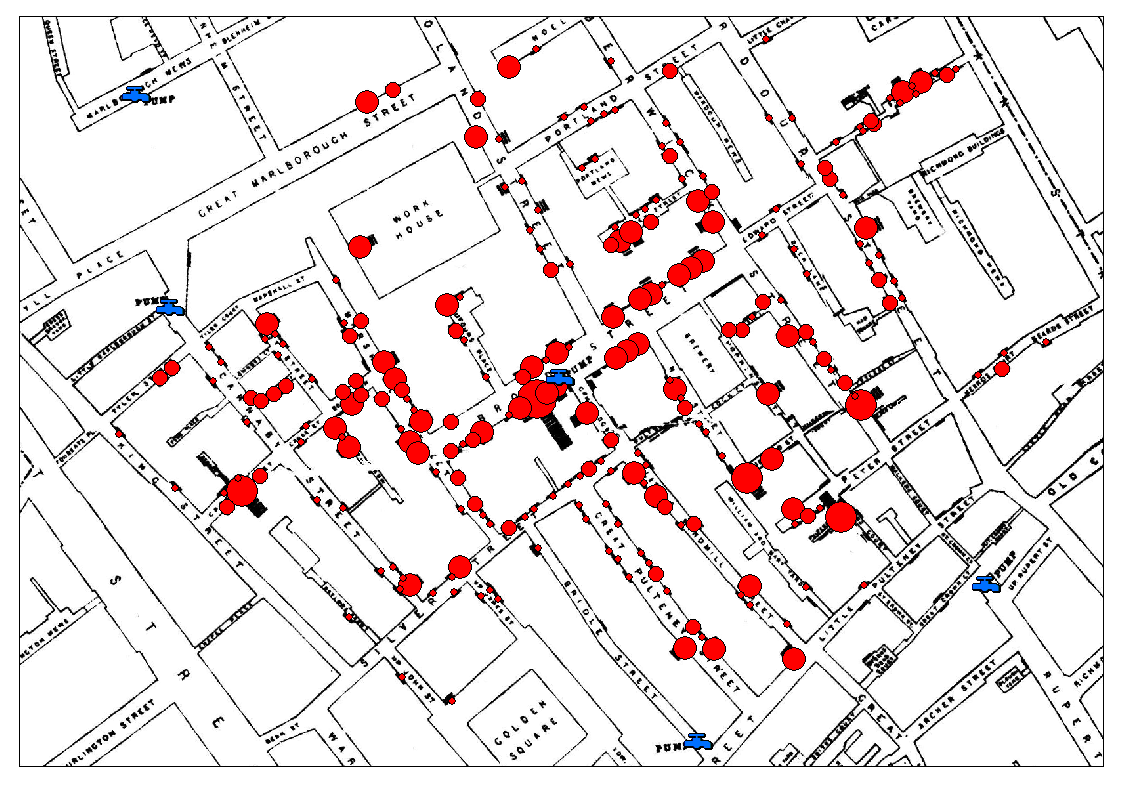
\includegraphics[width=1\linewidth]{graphs/SnowMap_Points.png}
\end{figure}
\end{center}
 }
 
\frame{ \frametitle{}
\begin{center}
\begin{figure}
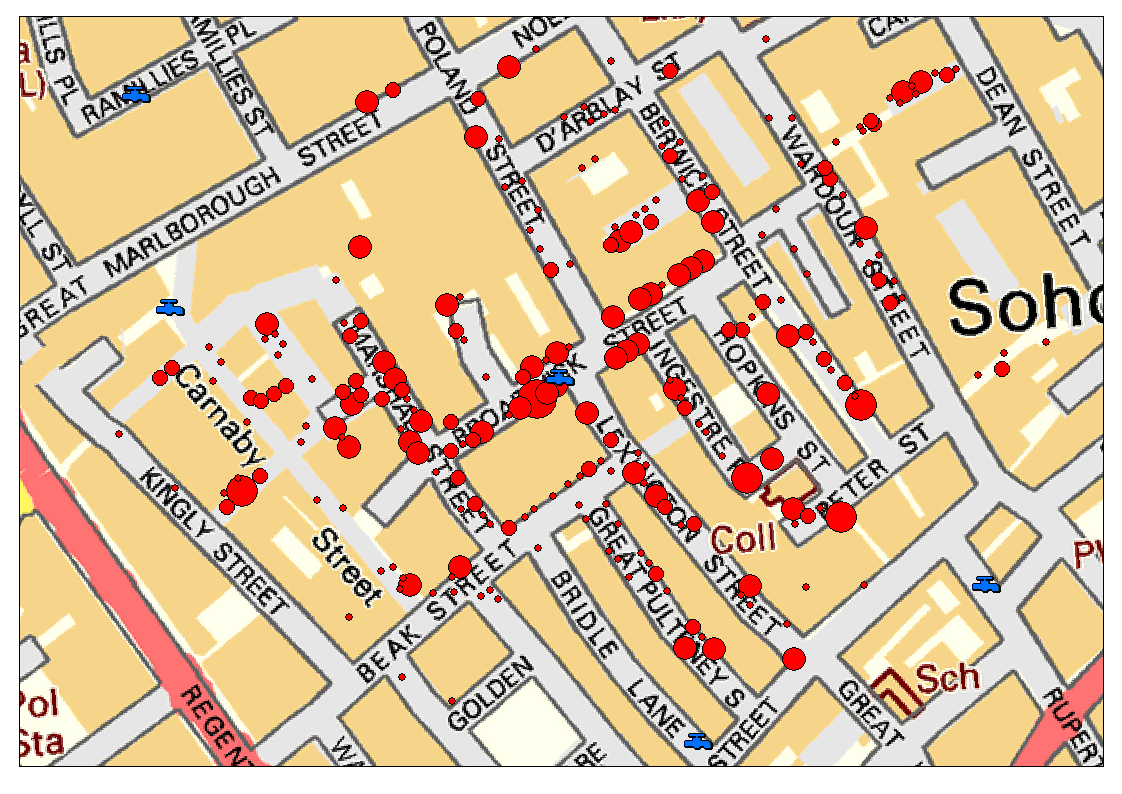
\includegraphics[width=1\linewidth]{graphs/OSColor_Points.png}
\end{figure}
\end{center}
 }
 

 
\frame{ \frametitle{}
\begin{center}
\begin{figure}[t]
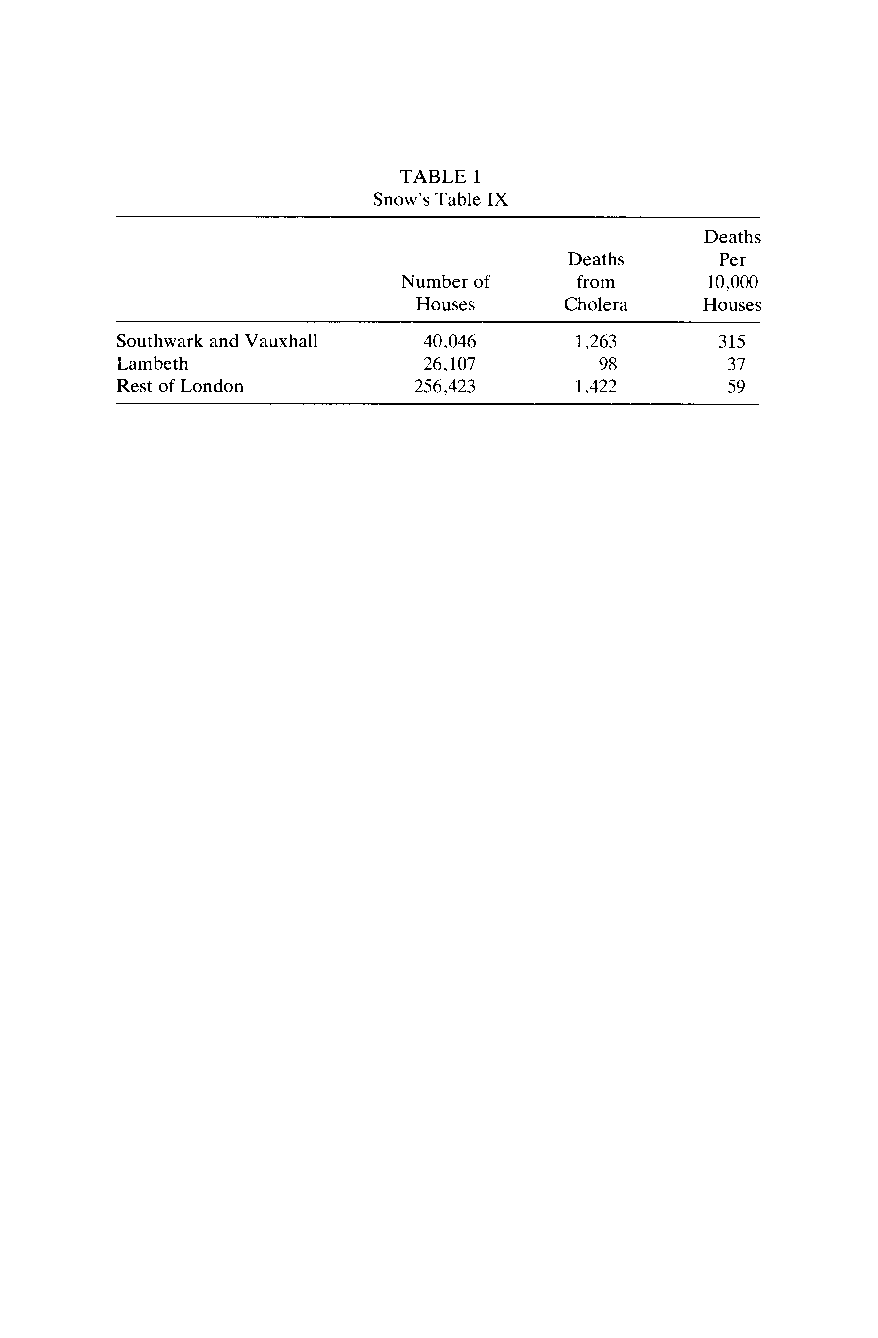
\includegraphics[width=1.1\linewidth]{graphs/freedman_tab1.pdf}
\end{figure}
\end{center}
 }

\begin{frame}
\frametitle{The Experimental Ideal}

Social experiment is the most influential research design. Why?
\bigskip

Solves Selection Problem
\end{frame}

\begin{frame}{Do hospitals make people healthier?}
\begin{itemize}
  \item Compare health status of people who were treated in hospital with those not treated in the average population
  \item Get data from National Health Interview Survey (NHIS)
  \item "During the last month, did you stay in hospital overnight?" Yes/No
  \item "Your health is": Excellent (1), very good (2), good (3), fair (4), poor (5)
  \item Selection: who is hospitalized?
\end{itemize}
\end{frame}



\frame{ \frametitle{}
\begin{center}
\begin{figure}[t]
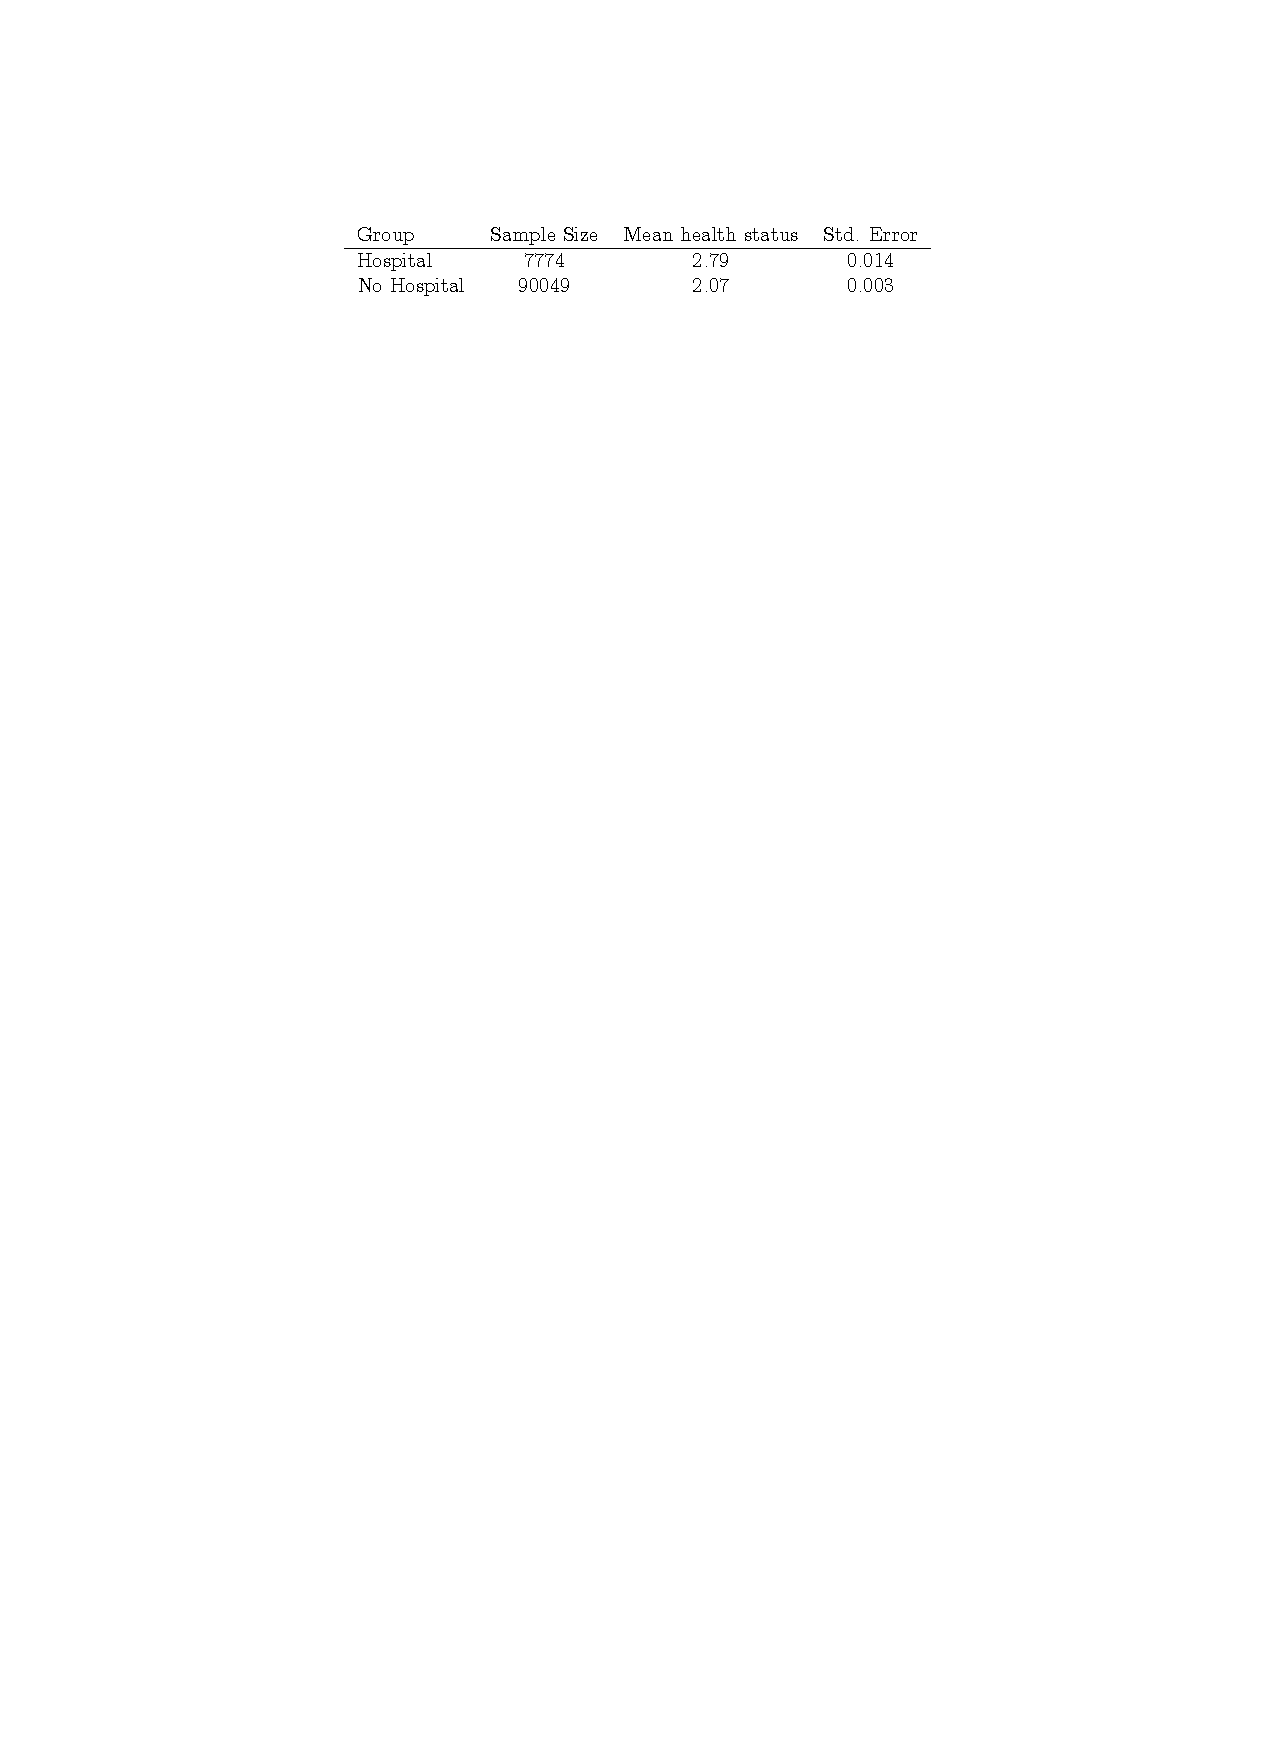
\includegraphics[width=1.1\linewidth]{graphs/ap_health.pdf}
\end{figure}
\end{center}
 }

   \begin{frame}
\frametitle{Potential Outcome Model}
$D_i=\{0,1 \}$ treatment variable (hospital care)

For each population unit $i$ we consider two \emph{potential outcomes} (health status)
\[\begin{array}{cl}
    Y_{1i} & \text{outcome with treatment} \\
    Y_{0i} & \text{outcome without treatment}
  \end{array}
\]
The gain from treatment or \emph{causal effect} for unit $i$ is
\[ Y_{i1}-Y_{i0} \]
Problem: For each $i$, only one of  $ Y_{i1}$ or $Y_{i0}$ is observed.

%\emph{Missing data problem}

\end{frame}

\begin{frame}
\frametitle{Observed outcome}

We observe
\begin{eqnarray*}
Y_i  &=& \left\{ \begin{array}{cc}
                                                Y_{1i} & \text{if}\;\; D_i=1 \\
                                                Y_{0i} & \text{if}\;\; D_i=0
                            \end{array}
                            \right. = Y_{0i}+ (Y_{1i}-Y_{0i}) D_i
\end{eqnarray*}


In the population distribution of $Y_{1i}$ and $Y_{0i}$, we can compare the average health of \emph{treated} and \emph{non-treated}


\begin{eqnarray*}
  \underset{\text{observed difference}}{\underbrace{E(Y_i|D_i=1)-E(Y_i|D_i=0)}} &=&  \\
  \underset{\text{average treatment effect}}{\underbrace{E(Y_{1i}|D_i=1)-E(Y_{0i}|D_i=1)}}  &+& \underset{\text{selection bias}}{\underbrace{E(Y_{0i}|D_i=1)-E(Y_{0i}|D_i=0) }}
\end{eqnarray*}

\end{frame}


\begin{frame}
\frametitle{Random assignment as a solution}

Random assignment makes $D_i$ independent of the potential outcome
\begin{eqnarray*}
E(Y_i|D_i=1)-E(Y_i|D_i=0)  &=& E(Y_{1i}|D_i=1)-E(Y_{0i}|D_i=0) \\
        &=& E(Y_{1i}|D_i=1)-E(Y_{0i}|D_i=1)  \\
         &=& E(Y_{1i}-Y_{0i}|D_i=1)=E(Y_{1i}-Y_{0i})  \\
\end{eqnarray*}
The observed difference in mean outcomes equals the \emph{average treatment effect}.

Examples:
\begin{itemize}
  \item health treatments
  \item government sponsored training programs
  \item education production: effect of class size, teacher quality, etc. on  student achievement
\end{itemize}

\end{frame}

   \frame{ \frametitle{Cameron et al (2016): RCT in
development}
\begin{center}
\begin{figure}[t]
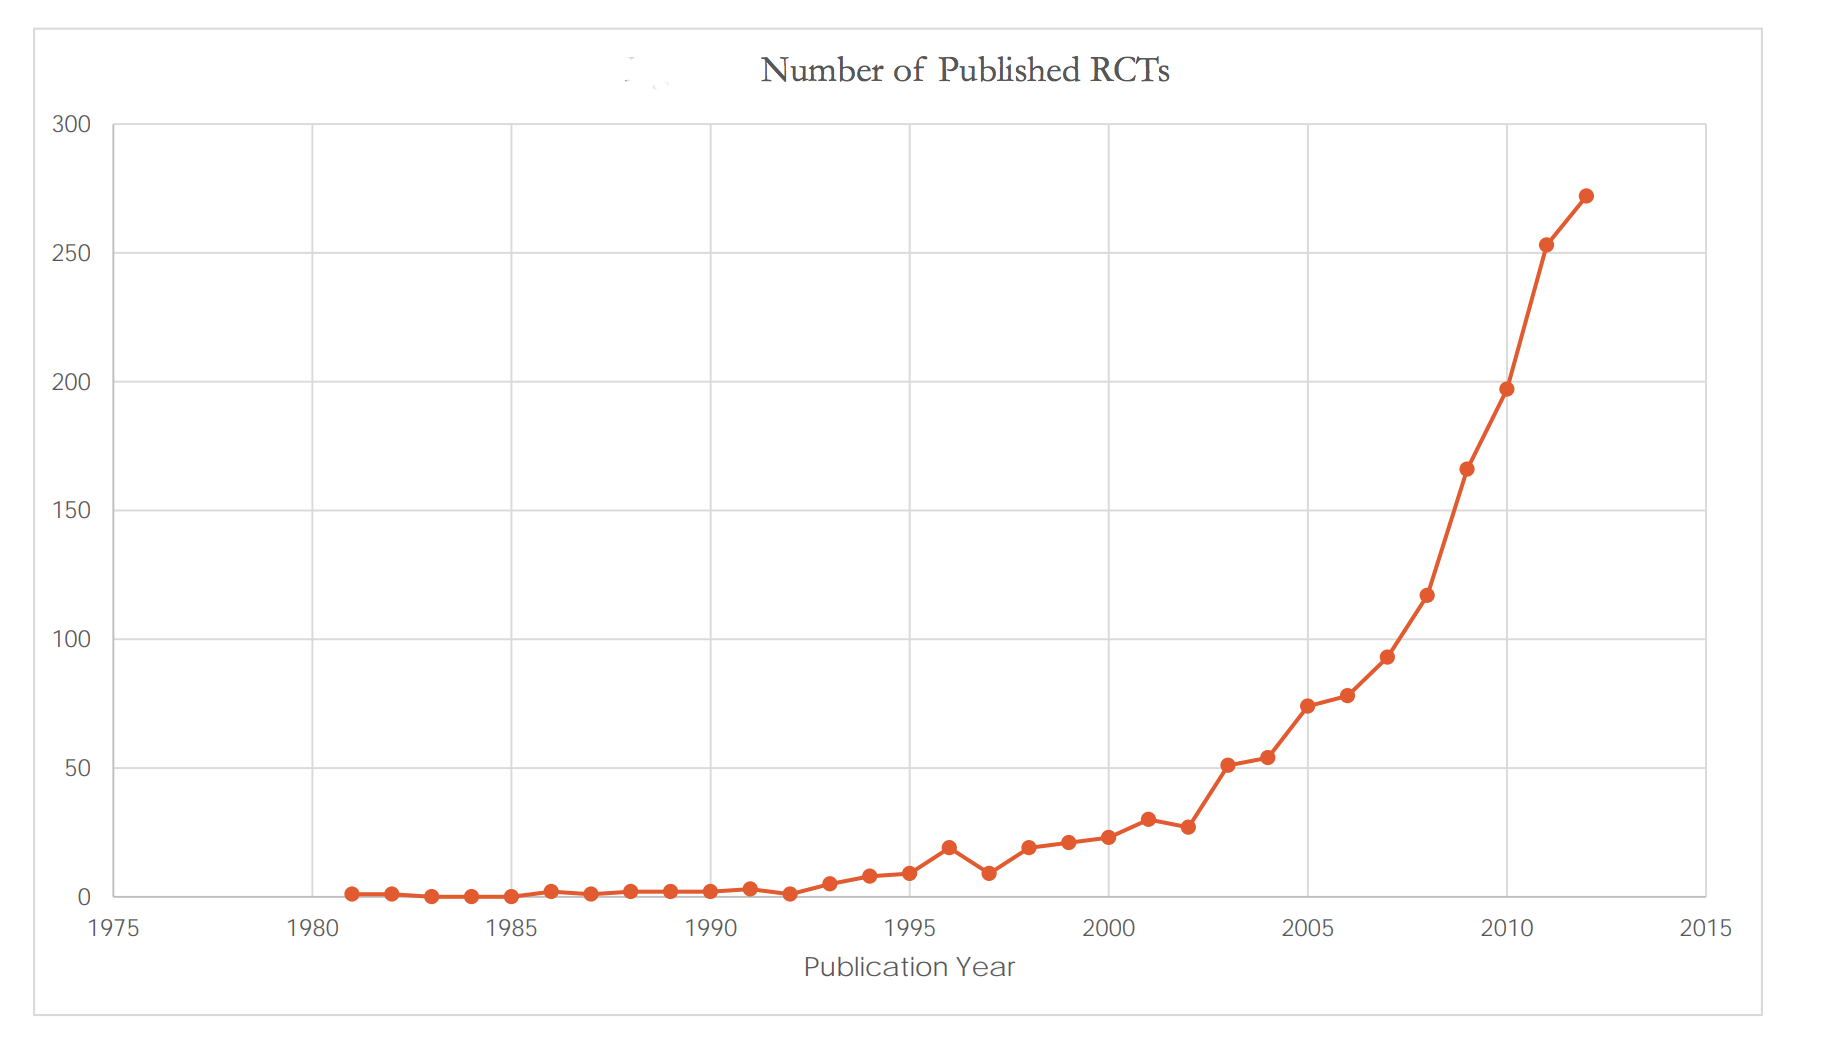
\includegraphics[width=1.0\linewidth]{graphs/rct_economics.png}
\end{figure}
\end{center}
 }

\begin{frame}
\frametitle{STAR Experiment}
Large randomized experiment involving 11,600 children in 1985-86, who were followed over 4 years
\bigskip

Treatment:
\begin{itemize}
  \item small classes: 13-17 kids
  \item regular classes: 22-25 kids
  \item regular classes with teacher aid
\end{itemize}
Successful randomization: Subjects' socioeconomic background characteristics balanced across treatment groups

\end{frame}

   \frame{ \frametitle{}
\begin{center}
\begin{figure}[t]
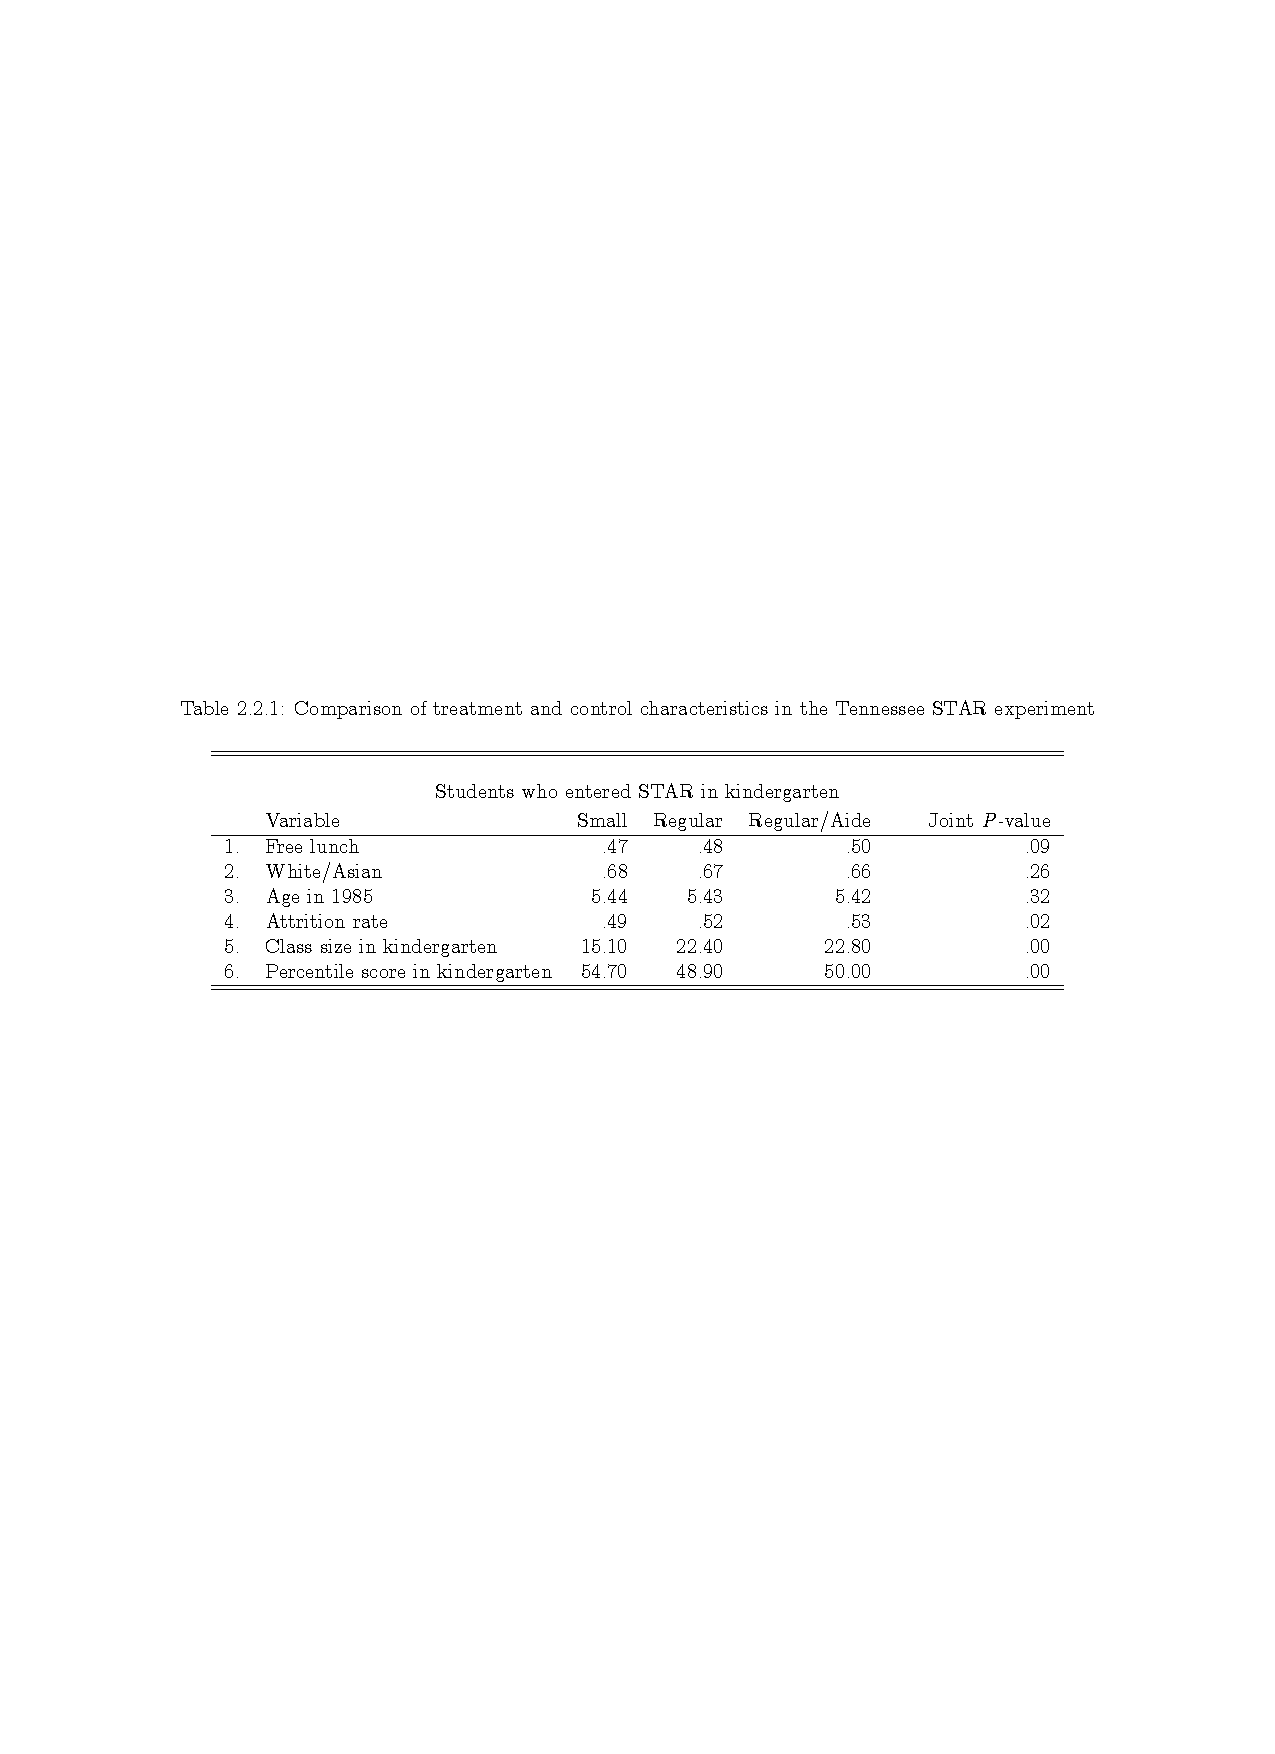
\includegraphics[width=1.0\linewidth]{graphs/ap_tab221.pdf}
\end{figure}
\end{center}
 }

\frame{ \frametitle{}
\begin{center}
\begin{figure}[t]
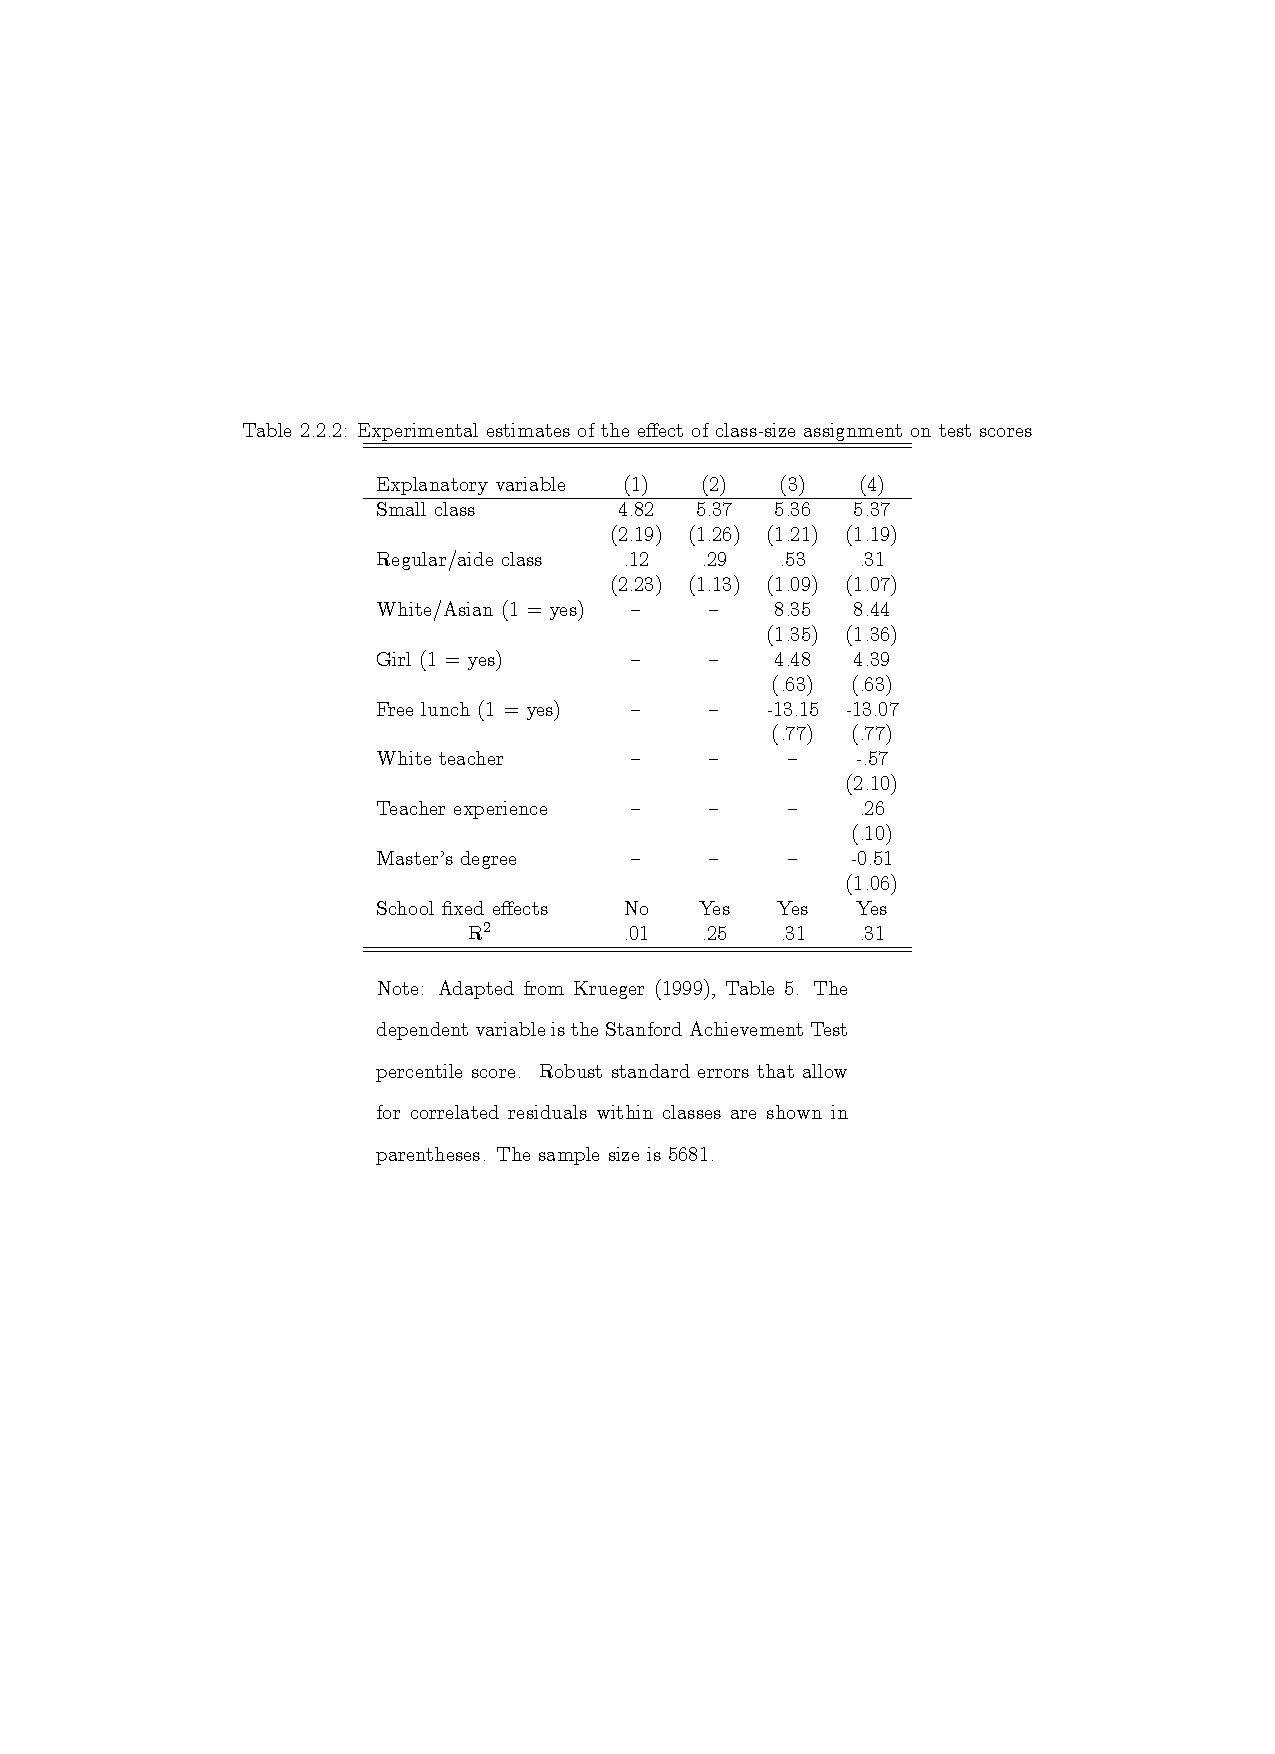
\includegraphics[width=1.0\linewidth]{graphs/ap_tab222.pdf}
\end{figure}
\end{center}
 }
 
 \begin{frame}
\frametitle{Regression Analysis of Experiments}
Assume $Y_{i1}-Y_{i0} = \rho$ \emph{constant} treatment effect
\begin{eqnarray*}
 Y_i &=&  \alpha + \rho D_i + \eta_i
\end{eqnarray*}

\begin{eqnarray*}
 E(Y_i|D_i=1) &=&  \alpha + \rho  +  E(\eta_i|D_i=1) \\
 E(Y_i|D_i=0) &=&  \alpha  +  E(\eta_i|D_i=0) \\
 E(Y_i|D_i=1)-E(Y_i|D_i=0)&=&    \rho +  \underset{\text{selection bias}}{\underbrace{E(\eta_i|D_i=1)-E(\eta_i|D_i=0)}}
\end{eqnarray*}
Selection bias amounts to correlation between regression error $\eta_i$ and $D_i$.
\end{frame}




 \begin{frame}
\frametitle{Regression Analysis of Experiments}
We know about the selection bias
\begin{eqnarray*}
 E(\eta_i|D_i=1)-E(\eta_i|D_i=0)= E(Y_{0i}|D_i=1)-E(Y_{0i}|D_i=0)
\end{eqnarray*}
If $D_i$ is randomly assigned, the selection bias is equal to zero.

Thus estimating the regression model results in the \emph{causal effect} $\rho$.
\bigskip

Regression model with covariates
\begin{eqnarray*}
 Y_i &=&  \alpha + \rho D_i + \beta X_i+ \eta_i
\end{eqnarray*}
If $X_i$ uncorrelated with $D_i$, including them will not affect estimate of $\rho$, but increase precision.

\end{frame}

\frame{ \frametitle{}
\begin{center}
\begin{figure}[t]
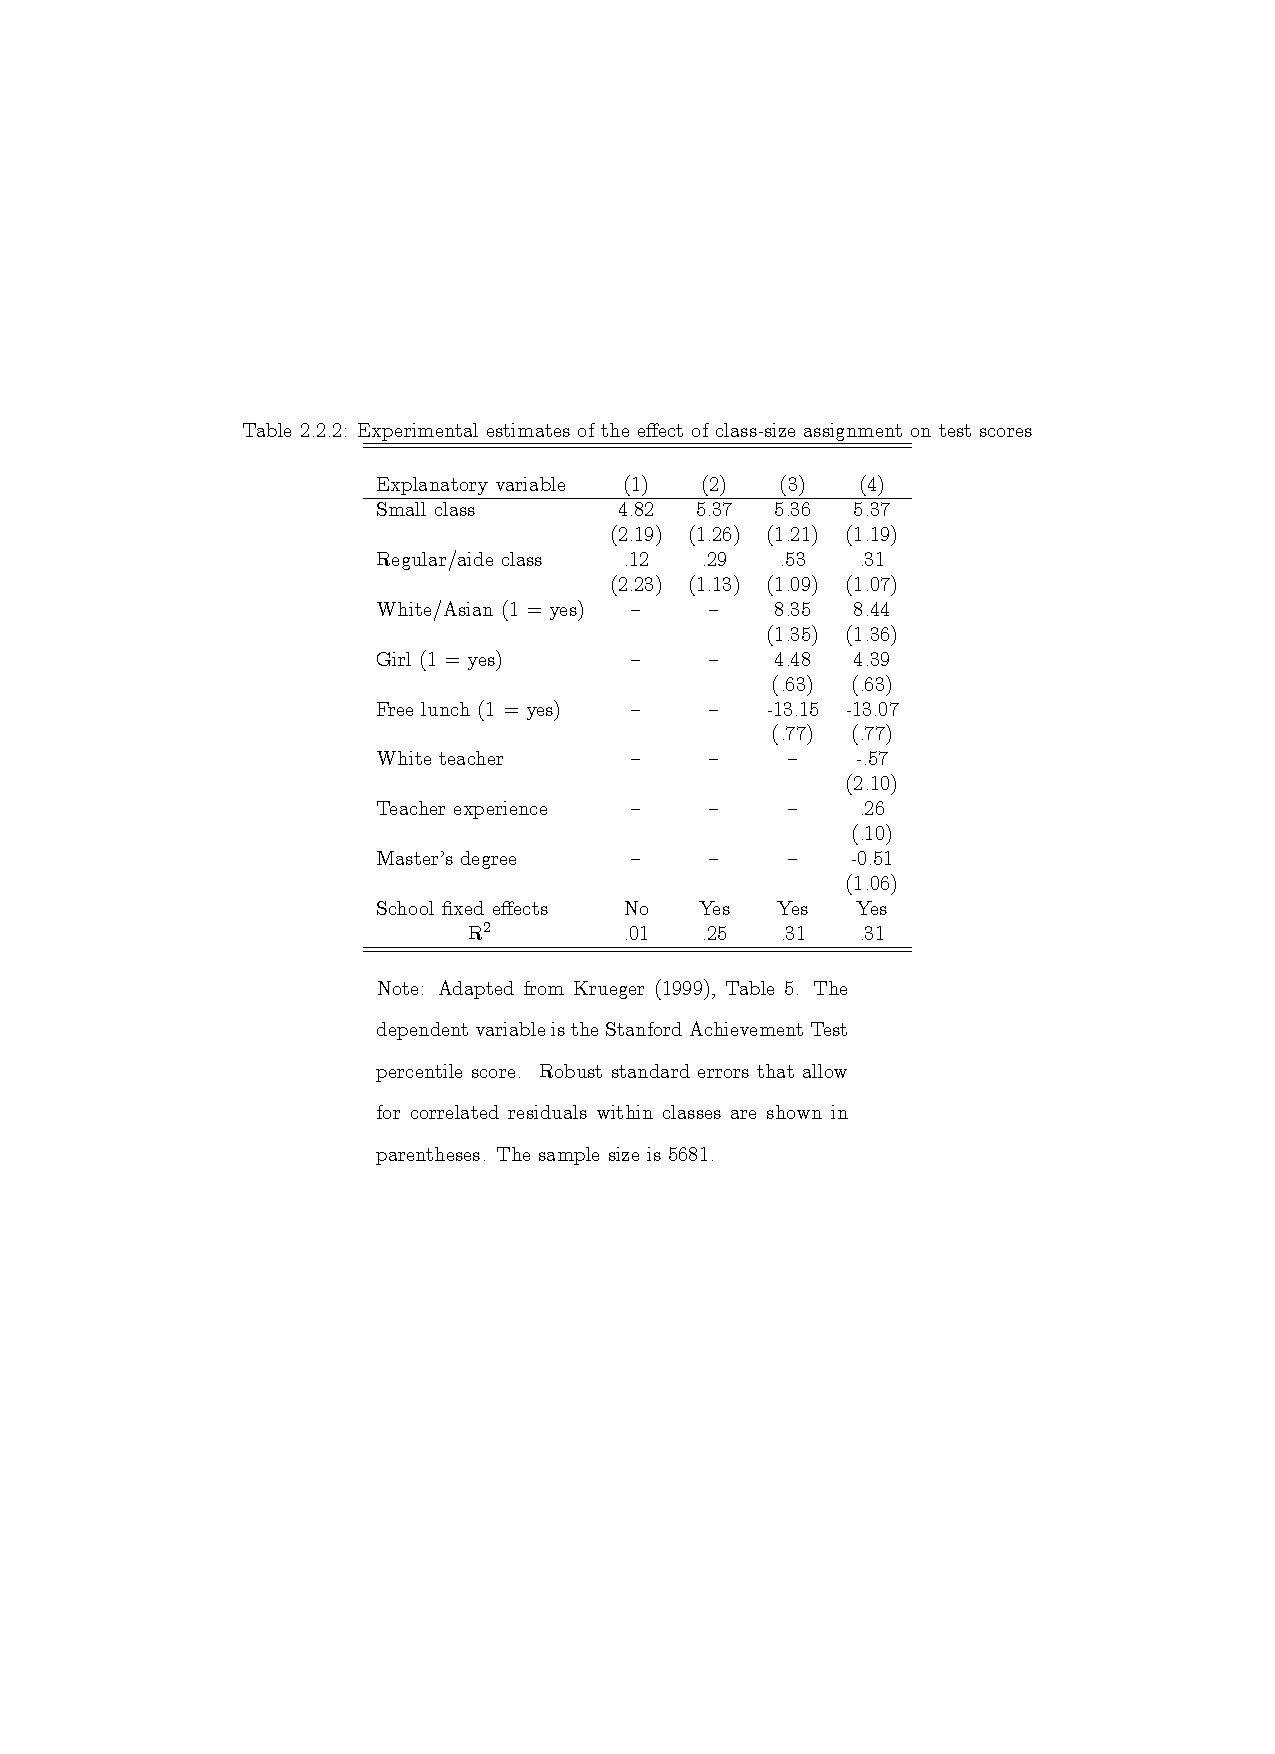
\includegraphics[width=1.0\linewidth]{graphs/ap_tab222.pdf}
\end{figure}
\end{center}
 }
\end{document}


